These requirements are likely unfeasible. In order to obtain a test whose true-positive rate is 0.97, the true-negative rate would have to be nearly 1 (see Figure \ref{fig:tpr}).

\begin{figure}[H]
    \centering
    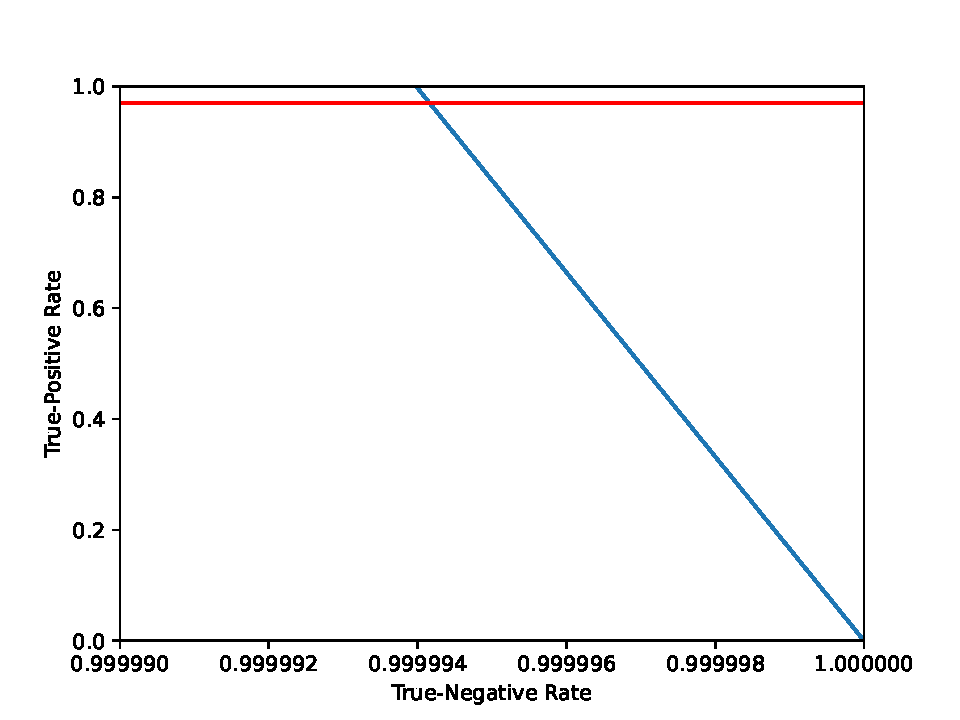
\includegraphics[width=0.8\linewidth]{images/tpr.pdf}
    \caption{Theoretical true-positive rate versus true-negative rate.}
    \label{fig:tpr}
\end{figure}

